\sectionquestion{Perceptron}

\begin{parts}



        \part[2] \textbf{Select all that apply:} Which of the following statements is true for the convergence of a perceptron on a binary classification problem:
        {%
        \checkboxchar{$\Box$} \checkedchar{$\blacksquare$} % change checkbox style locally]
        \begin{checkboxes}
            \choice If the batch perceptron learning algorithm converges, the number of mistakes it makes before convergence depends on the order in which data points are seen. 
            \choice Whether or not the batch perceptron learning algorithm converges depends on the order in which data points are seen. 
            \choice The batch perceptron learning algorithm will make a bounded number of mistakes if the training dataset is not linearly separable.
            \choice The batch perceptron learning algorithm will loop forever if the training dataset is not linearly separable.
            \choice None of the above
        \end{checkboxes}
        }
        \begin{soln}
        A - order affects the mistakes the perceptron makes \& D - the perceptron does not converge on data that is not linearly separable.
        \end{soln}
        \begin{qauthor}
        Author: Aditi Sharma
        Objective: Determine whether the perceptron algorithm will converge based on properties of the dataset, and the limitations of the convergence guarantees
        
        Edited by Henry
        \end{qauthor}

        \begin{qtester}
        EA Feedback: I like this question. I wonder if we should specify that there is no stopping condition other than convergence or something. But I also don't want to make it too obvious. 
        \end{qtester}

\part[1] \textbf{True or False:} In classification, online learning differs from batch learning in that the former aims to minimizes the number of mistakes it makes on the training examples, whereas the latter aims to minimize mistakes on a fixed set of held out examples.
    \begin{checkboxes}
     \choice True 
     \choice False
    \end{checkboxes}
    \begin{soln}
    True
    \end{soln}
    \begin{qauthor}
    Matt
    \end{qauthor}


\part[4] \textbf{Select all that apply:} Which of the following datasets is linearly separable?

\begin{minipage}{0.3\linewidth}
\textit{Dataset A:}\\
\begin{tabular}{ccc}
     $x_1$ & $x_2$ & $y$ \\
     \midrule
     -2 & -2 & -1 \\
     -1 & -1 & -1 \\
     0 & 0 & +1 \\
     1 & 1 & +1 \\
     2 & 2 & +1 \\
\end{tabular}
\end{minipage}
%
\begin{minipage}{0.3\linewidth}
\textit{Dataset B:}\\
\begin{tabular}{ccc}
     $x_1$ & $x_2$ & $y$ \\
     \midrule
     0 & 0 & -1 \\
     1 & 1 & -1 \\
     0 & 1 & +1 \\
     1 & 0 & +1 \\
\end{tabular}
\end{minipage}
%
\begin{minipage}{0.3\linewidth}
\textit{Dataset C:}\\
\begin{tabular}{cccc}
     $x_1$ & $x_2$ & $x_3$ & $y$ \\
     \midrule
     2 & 0 & 0 & -1 \\
     3 & 1 & 1 & -1 \\
     2 & 1 & 0 & -1 \\
     1 & 0 & 3 & +1 \\
     1 & 2 & 1 & +1 \\
     2 & 2 & 2 & +1 \\
\end{tabular}
\end{minipage}
    {%
    \checkboxchar{$\Box$} \checkedchar{$\blacksquare$} % change checkbox style locally
    \begin{checkboxes}
     \choice Dataset A
     \choice Dataset B
     \choice Dataset C
     \choice None of the above
    \end{checkboxes}
    }
    \begin{soln}
    Dataset A and Dataset C
    \begin{itemize}
        \item A: really just a line (extra feature is a copy)
        \item B: XOR
        \item C: example solution $\wv = [-1, 1, 1], b = 0$
    \end{itemize}
    Points: correctness on A is worth 1 pt, correctness on B is 1 pt, correctness on C is 2 pts.
    \end{soln}
    \begin{qauthor}
    Matt
    \end{qauthor}

\clearpage

\part Suppose you are given a linear decision boundary defined by weight vector $\wv = [10, -8]^T$ and intercept $b = 0$. \emph{(Note: For each question below, draw your answer on the provided axes and clearly label each part.)}

%\begin{figure}[H]
    \begin{center}
    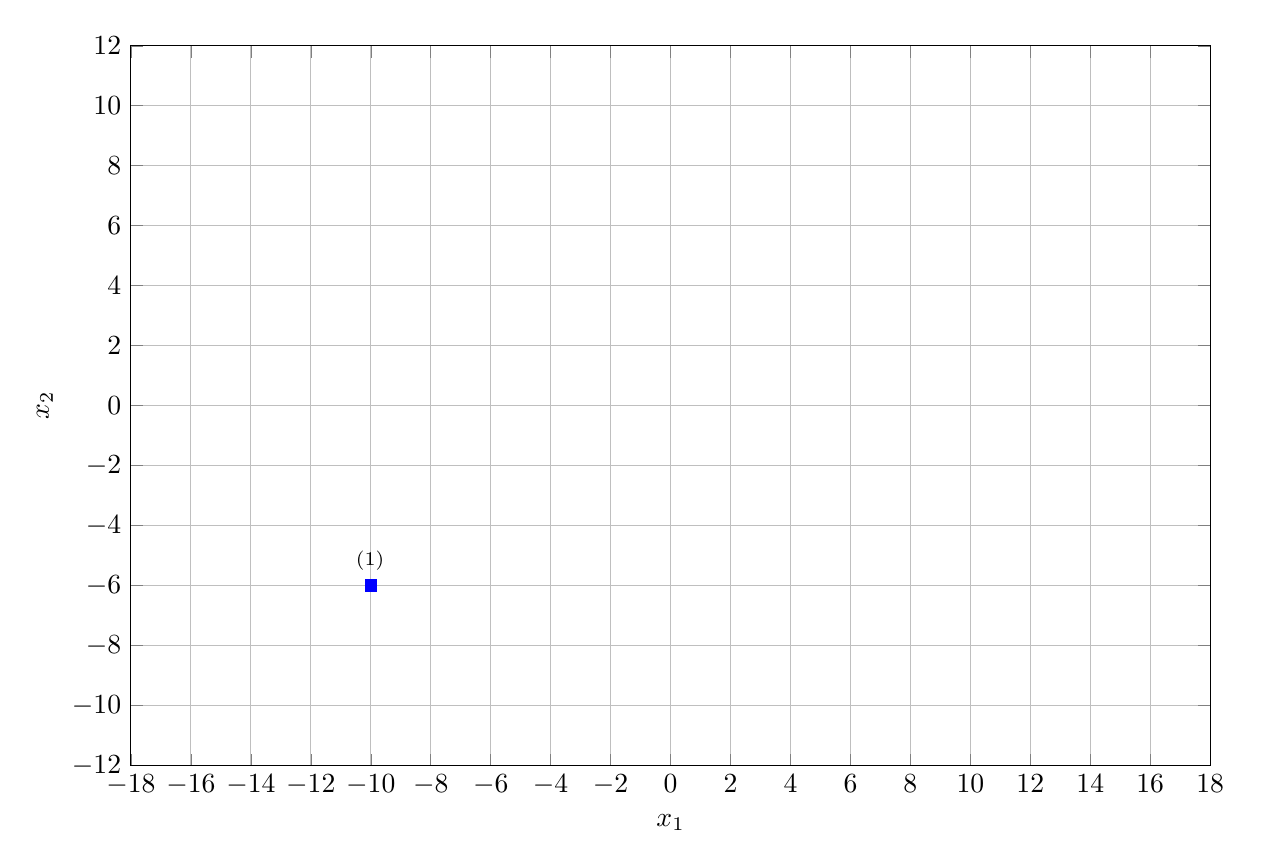
\begin{tikzpicture}
    \begin{axis}[
        scale=2.0, axis equal image,
        xmin=-18, xmax=18, xtick={-18,-16,...,18},
        ymin=-12, ymax=12, ytick={-12,-10,...,12},
        samples=50, grid=major, xlabel=$x_1$, ylabel=$x_2$]
        %\addplot[blue, ultra thick] (x,x*x);
        %\addplot[red,  ultra thick] (x*x,x);
        \addplot [
            scatter,
            only marks,
            point meta=explicit symbolic,
            scatter/classes={
                a={mark=square*,blue},
                b={mark=triangle*,red}
            },
            nodes near coords*={$\xv^{(\pgfmathprintnumber[frac]\myvalue)}$},
            visualization depends on={\thisrow{myvalue} \as \myvalue},
        ] table [meta=label] {
            x y label myvalue
            -10 -6 a 1
        };
    \end{axis}
    \end{tikzpicture}
    \end{center}
   % \caption{}
%    \label{fig:percdata}
%\end{figure}

\begin{subparts}

\subpart[1] Draw the weight vector $\wv$.

\subpart[2] Draw the decision boundary.

\subpart[1] \textbf{Select one:} Would this classifier correctly or incorrectly classify the point shown as $\xv^{(1)}$ if its true label is $y^{(1)} = +1$?
    \begin{checkboxes}
     \choice correctly classify
     \choice incorrectly classify
    \end{checkboxes}
    \begin{soln}
    Incorrectly classify
    \end{soln}
    \begin{qauthor}
    Matt
    \end{qauthor}

\subpart[2] Suppose the intercept $b$ is decreased to some new value such that $b < 0$. Draw an arrow pointing in the exact direction that the decision boundary will move, relative to its current position.
    \begin{soln}
    Arrow pointing down and/or right (in the direction of w)
    \end{soln}
    \begin{qauthor}
    Matt
    \end{qauthor}
\subpart[2] Briefly justify why, in a Perceptron, subtracting one from the value of $b$ when we make a mistake and the label is negative is a sensible adjustment to the parameters.
    \fillwithlines{6em}
    \begin{soln}
    Subtracting one will move the decision boundary towards (the avg. of) those positive points on which Perceptron previously made a mistake and away from (the avg. of) those negative points on which it made mistake, thus creating more space on the negative side relative to the previous decision boundary before said intercept adjustment.
    \end{soln}
    \begin{qauthor}
    Matt
    \end{qauthor}
\end{subparts}

\part You train a Perceptron classifier to determine whether a bug is a spotted lantern fly ($y = -1$) or a monarch butterfly ($y = +1$) based on $M = 4$ features that are readings from a robot's sensors.

After training for six iterations your have parameters:
\begin{align*}
    \wv = [-2, 3, 1, -1]^T && b = -1
\end{align*}
Your next training example is:
\begin{align*}
    \xv^{(7)} = [1, 1, 0, 1]^T && y^{(7)} = +1
\end{align*}

\begin{subparts}

\subpart[2] \textbf{Select one:} How does the Perceptron classifier label $\xv^{(7)}$?
    \begin{checkboxes}
     \choice $\hat{y} = -1$
     \choice $\hat{y} = +1$
    \end{checkboxes}
    \begin{soln}
    $\hat{y} = -1$
    \end{soln}
    \begin{qauthor}
    Matt
    \end{qauthor}

\subpart[3] \textbf{Numerical answer:} What are the parameters at the start of the next iteration?

     $w_1 = $ \begin{tcolorbox}[fit,height=1cm, width=2cm, blank, borderline={1pt}{-2pt}, nobeforeafter=false]
    %solution
    \end{tcolorbox}
    
     $w_2 = $ \begin{tcolorbox}[fit,height=1cm, width=2cm, blank, borderline={1pt}{-2pt}, nobeforeafter=false]
    %solution
    \end{tcolorbox}
    
     $w_3 = $ \begin{tcolorbox}[fit,height=1cm, width=2cm, blank, borderline={1pt}{-2pt}, nobeforeafter=false]
    %solution
    \end{tcolorbox}
    
     $w_4 = $ \begin{tcolorbox}[fit,height=1cm, width=2cm, blank, borderline={1pt}{-2pt}, nobeforeafter=false]
    %solution
    \end{tcolorbox}
    
     $b = $ \begin{tcolorbox}[fit,height=1cm, width=2cm, blank, borderline={1pt}{-2pt}, nobeforeafter=false]
    %solution
    \end{tcolorbox}
    \begin{soln}
    \begin{align*}
        \wv = [-1, 4, 1, 0]^T && b = 0
    \end{align*}
    1 point for $b$, half point for each $w_m$
    \end{soln}
    \begin{qauthor}
    Matt
    \end{qauthor}
    
\end{subparts}

\end{parts}